% !TeX root = ..\main.tex
\section{Thực thi quy trình nghiệp vụ}

\subsection{Thay đổi quy trình nghiệp vụ trong hệ thống}
\begin{figure}[!htp]
    \centering
    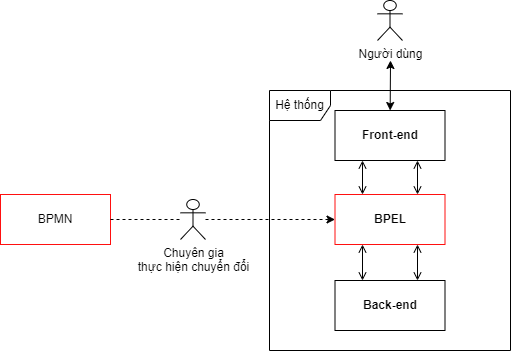
\includegraphics[width=10cm]{img/bpel/tranfer.png}
    \newline
    \caption{Cách thay đổi quy trình nghiệp vụ trong hệ thống}
\end{figure}

Đối với mỗi quy trình nghiệp vụ của hệ thống được thiết kế bằng BPMN, các chuyên gia cần thực hiện chuyền đổi các quy trình đó thành quy trình BPEL để thực thi và tích hợp vào hệ thông. Khi thực hiện thay đổi các quy trình nghiệp vụ trong hệ thống, chúng ta thực hiện thay đổi quy trình BPMN hiện có và chuyển đổi nó thành BPEL, từ đó hệ thống được cập nhật quy trình nghiệp vụ mà không cần thay đổi các thành phần khác trong hệ thống.


\subsection{Quy trình lấy danh sách sản phẩm}

\subsubsection*{Quy trình ban đầu}
\begin{figure}[!htp]
    \centering
    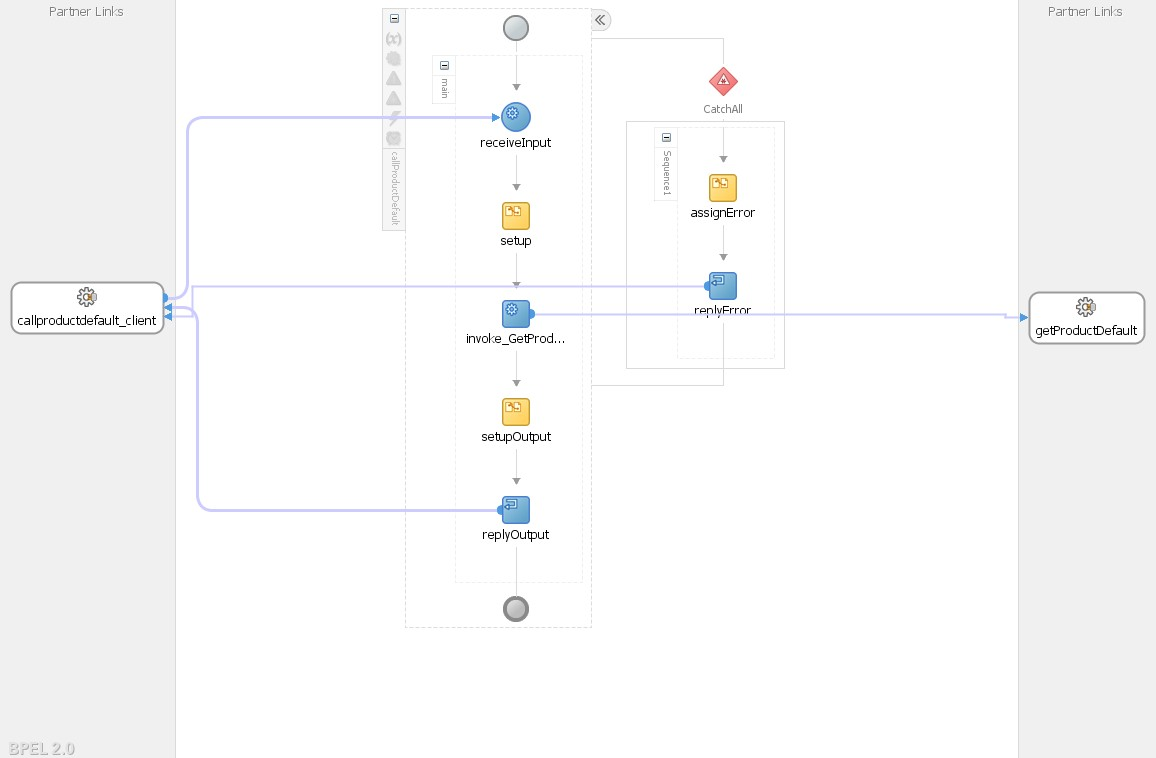
\includegraphics[width=12cm]{img/bpel/productDefault.jpg}
    \newline
    \caption{Quy trình lấy danh sách sản phẩm}
\end{figure}

\subsubsection*{Chuyển đổi quy trình}
Khi hệ thống được thêm event service, các sản phẩm được cập nhật lại giá bán, quy trình tính toán lại giá sản phẩm khi có event service như sau:
\begin{figure}[!htp]
    \centering
    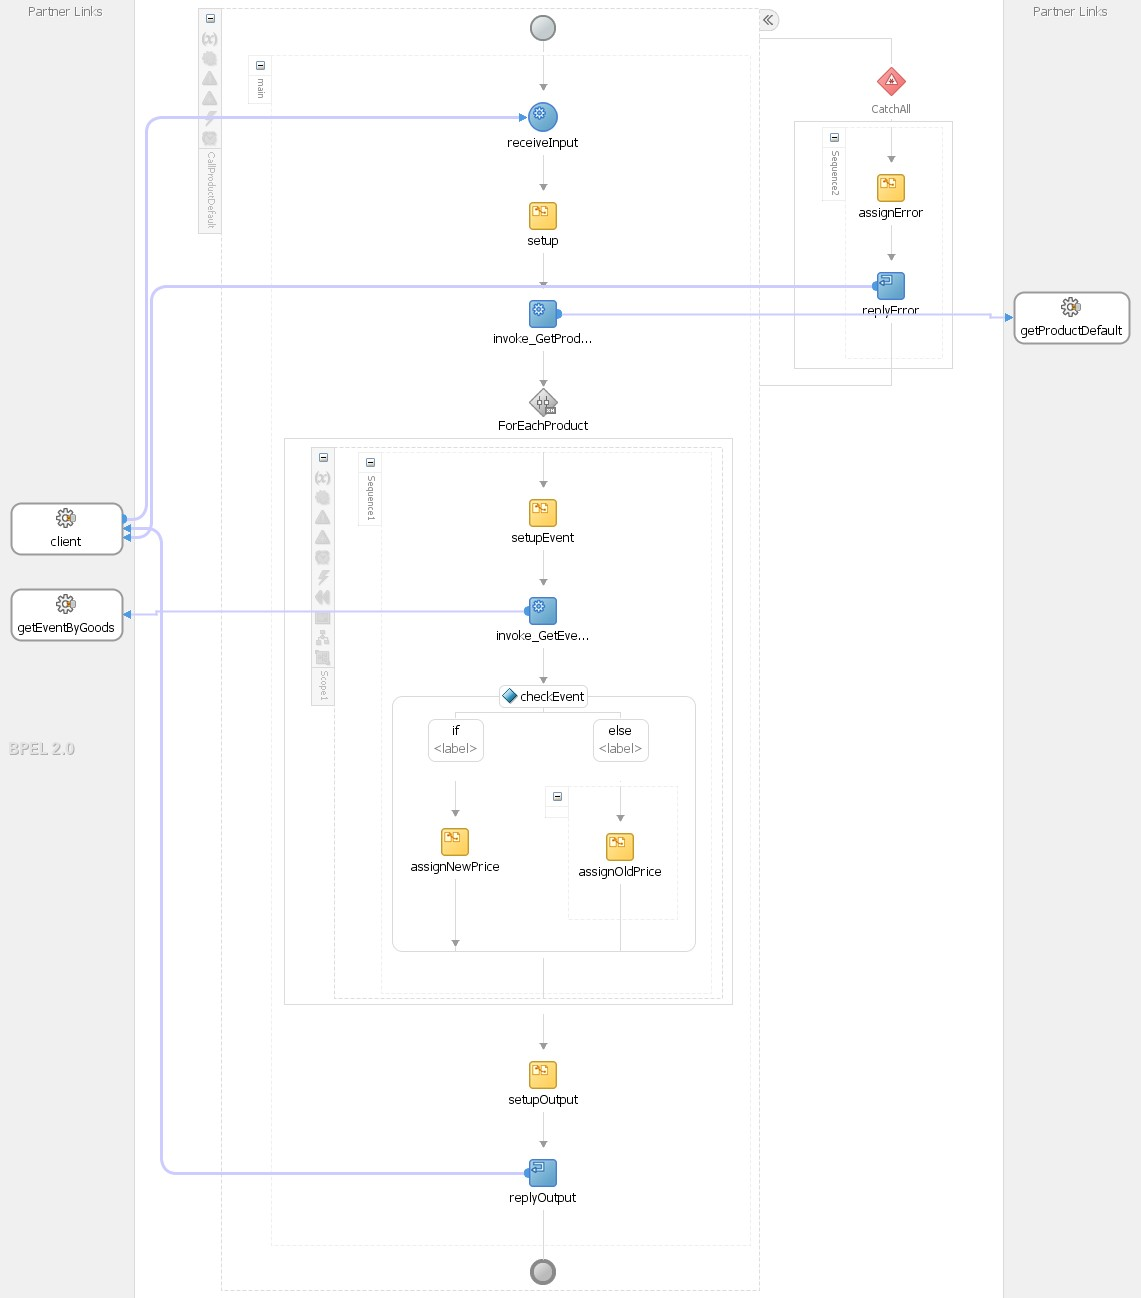
\includegraphics[width=14cm]{img/bpel/productDefaultAfter.jpg}
    \newline
    \caption{Quy trình lấy danh sách sản phẩm sau khi thay đổi}
\end{figure}

\newpage

\subsection{Quy trình lấy thông tin chi tiết sản phẩm}
\subsubsection*{Quy trình ban đầu}
\begin{figure}[!htp]
    \centering
    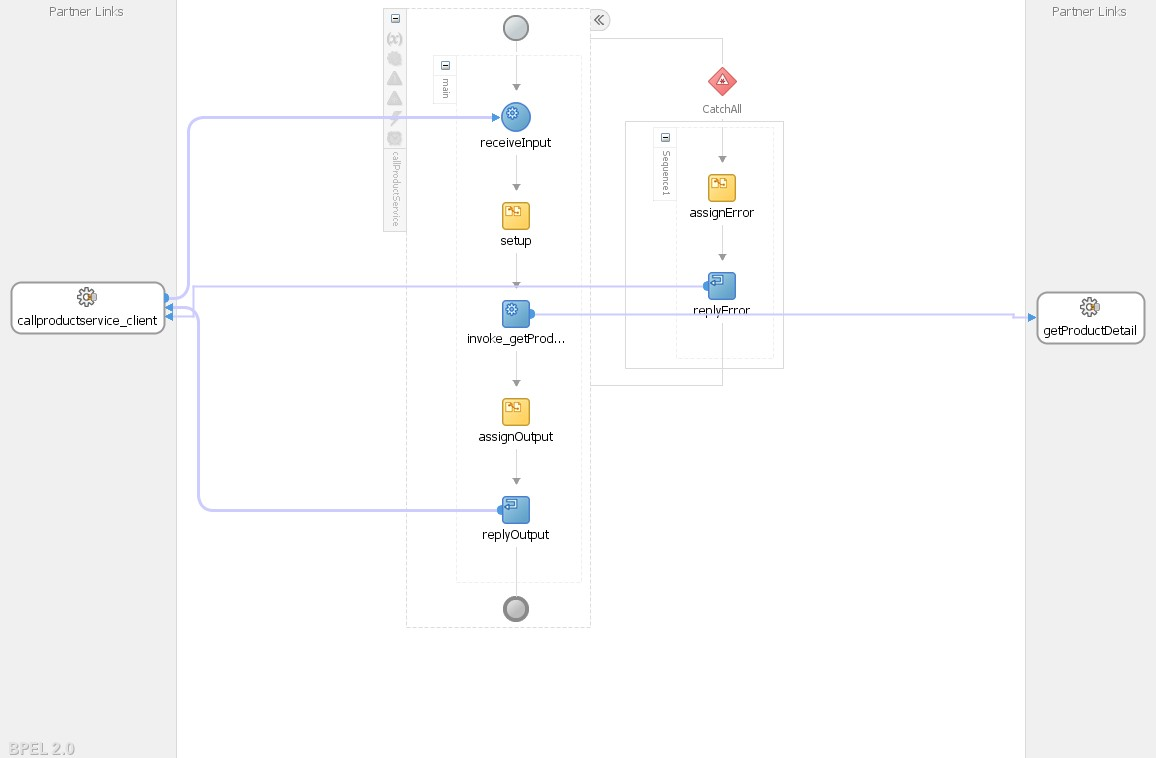
\includegraphics[width=12cm]{img/bpel/productDetail.jpg}
    \newline
    \caption{Quy trình lấy thông tin chi tiết sản phẩm}
\end{figure}

\subsubsection*{Chuyển đổi quy trình}
Khi hệ thống được thêm event service, các sản phẩm được cập nhật lại giá bán, quy trình tính toán lại giá sản phẩm khi có event service như sau:
\begin{figure}[!htp]
    \centering
    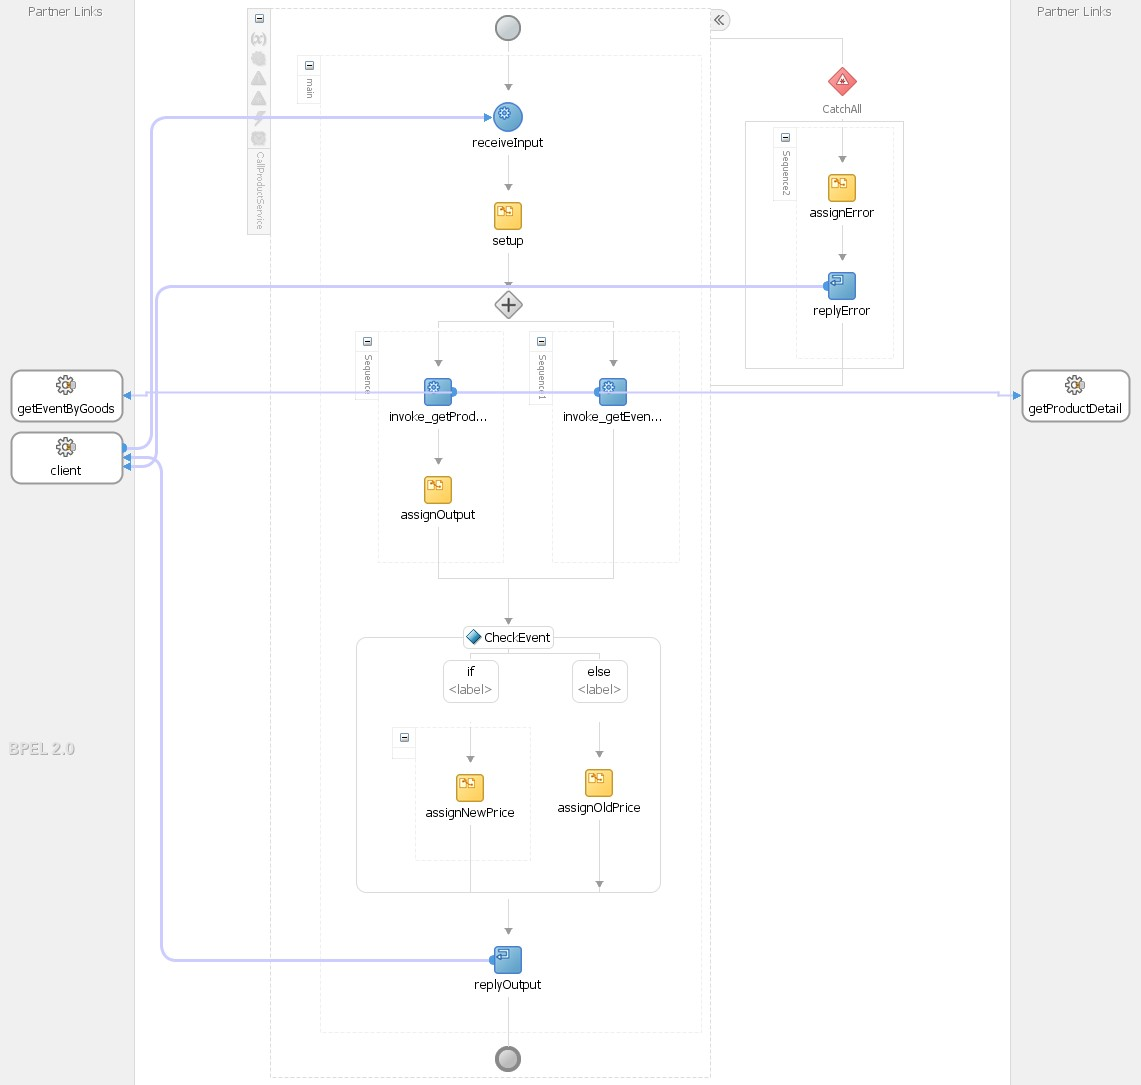
\includegraphics[width=14cm]{img/bpel/productDetailAfter.jpg}
    \newline
    \caption{Quy trình lấy thông tin chi tiết sản phẩm sau khi thay đổi}
\end{figure}

\newpage
\subsection{Quy trình tính giá giao hàng}
\subsubsection*{Quy trình ban đầu}
\begin{figure}[!htp]
    \centering
    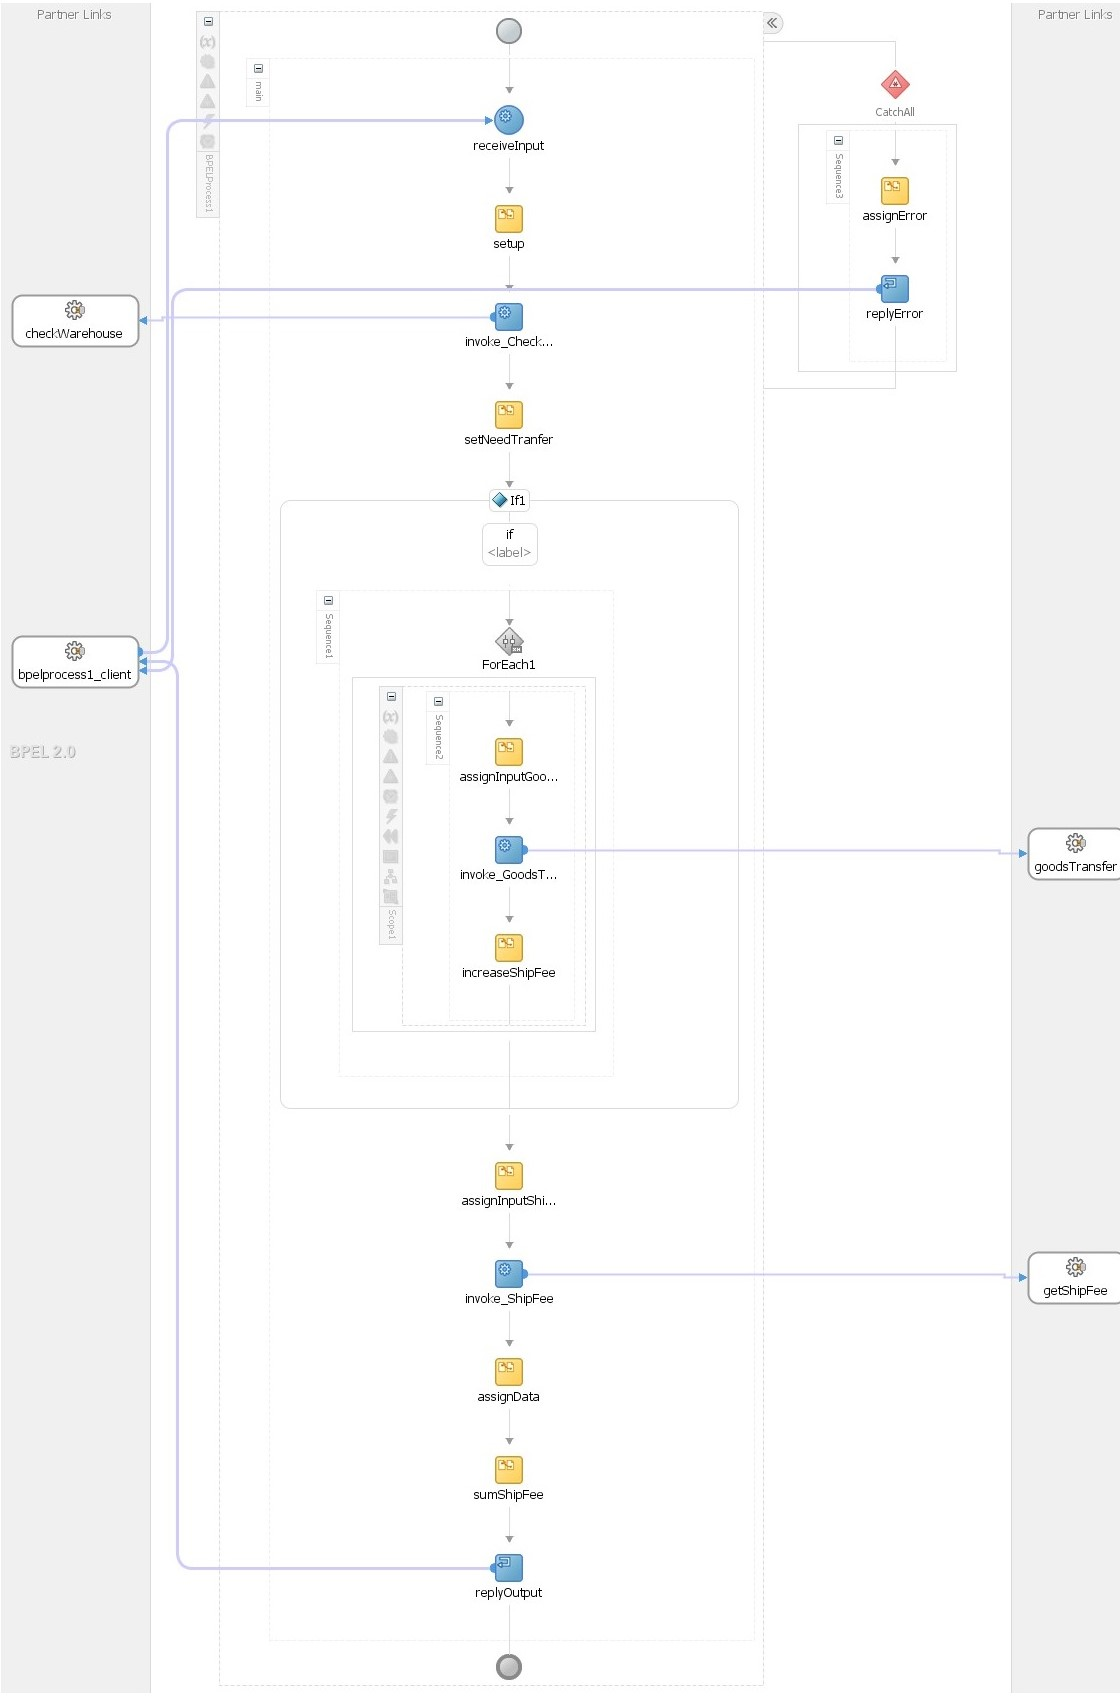
\includegraphics[width=14cm]{img/bpel/getShipFee.jpg}
    \newline
    \caption{Quy trình tính giá giao hàng}
\end{figure}
Giá giao hàng được tính toán dựa trên vị trí giao hàng của khách hàng cộng với chi phí vận chuyển hàng giữa các kho khi đơn hàng quá lớn

\subsubsection*{Chuyển đổi quy trình}
Sau khi doanh nghiệp chịu phí chuyển hàng giửa các kho khi đơn hàng lớn, phí giao hàng chỉ được tính toán dựa trên vị trí giao hàng của khách hàng. Quy trình được thay đổi bỏ đi việc tính toán chi phí chuyển kho như sau:
\begin{figure}[!htp]
    \centering
    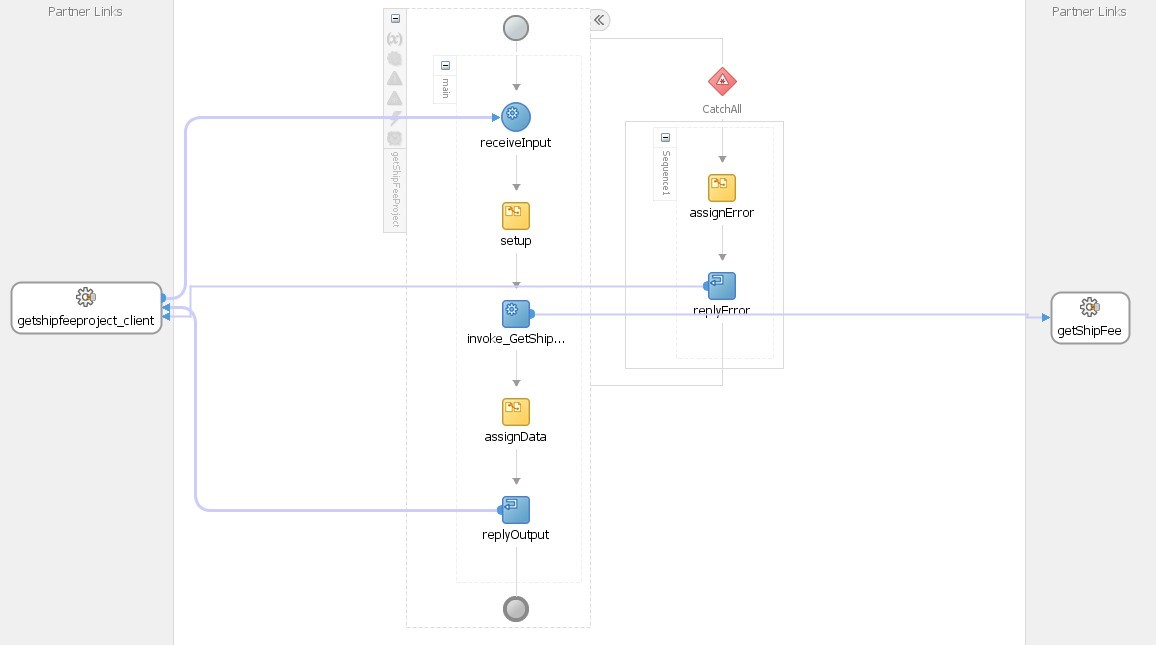
\includegraphics[width=12cm]{img/bpel/getShipFeeAfter.jpg}
    \newline
    \caption{Quy trình tính giá giao hàng sau khi thay đổi}
\end{figure}

\newpage
\subsection{Quy trình tạo đơn hàng}
\subsubsection*{Quy trình ban đầu}
\begin{figure}[!htp]
    \centering
    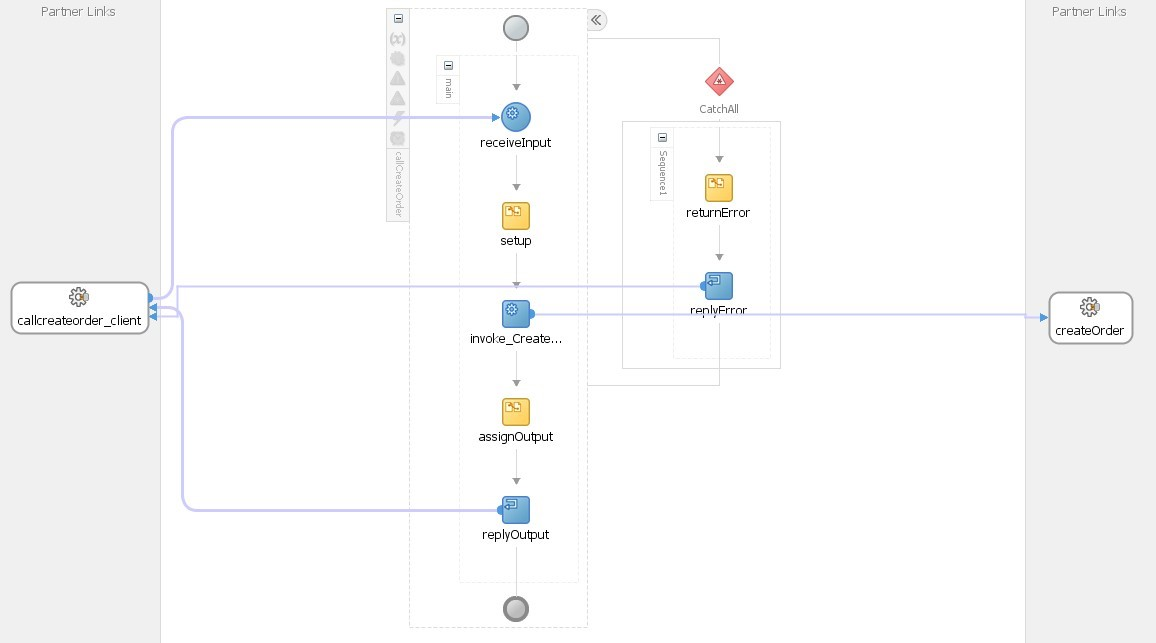
\includegraphics[width=12cm]{img/bpel/createOrder.jpg}
    \newline
    \caption{Quy trình tạo đơn hàng}
\end{figure}


\subsubsection*{Chuyển đổi quy trình}
Sau khi doanh nghiệp chịu phí chuyển hàng giửa các kho khi đơn hàng lớn, việc vận chuyển hàng giửa các kho được thực hiện sau khi khách hàng chốt đơn hàng. Quy trình được thay đổi bổ xung việc chuyển kho như sau:
\begin{figure}[!htp]
    \centering
    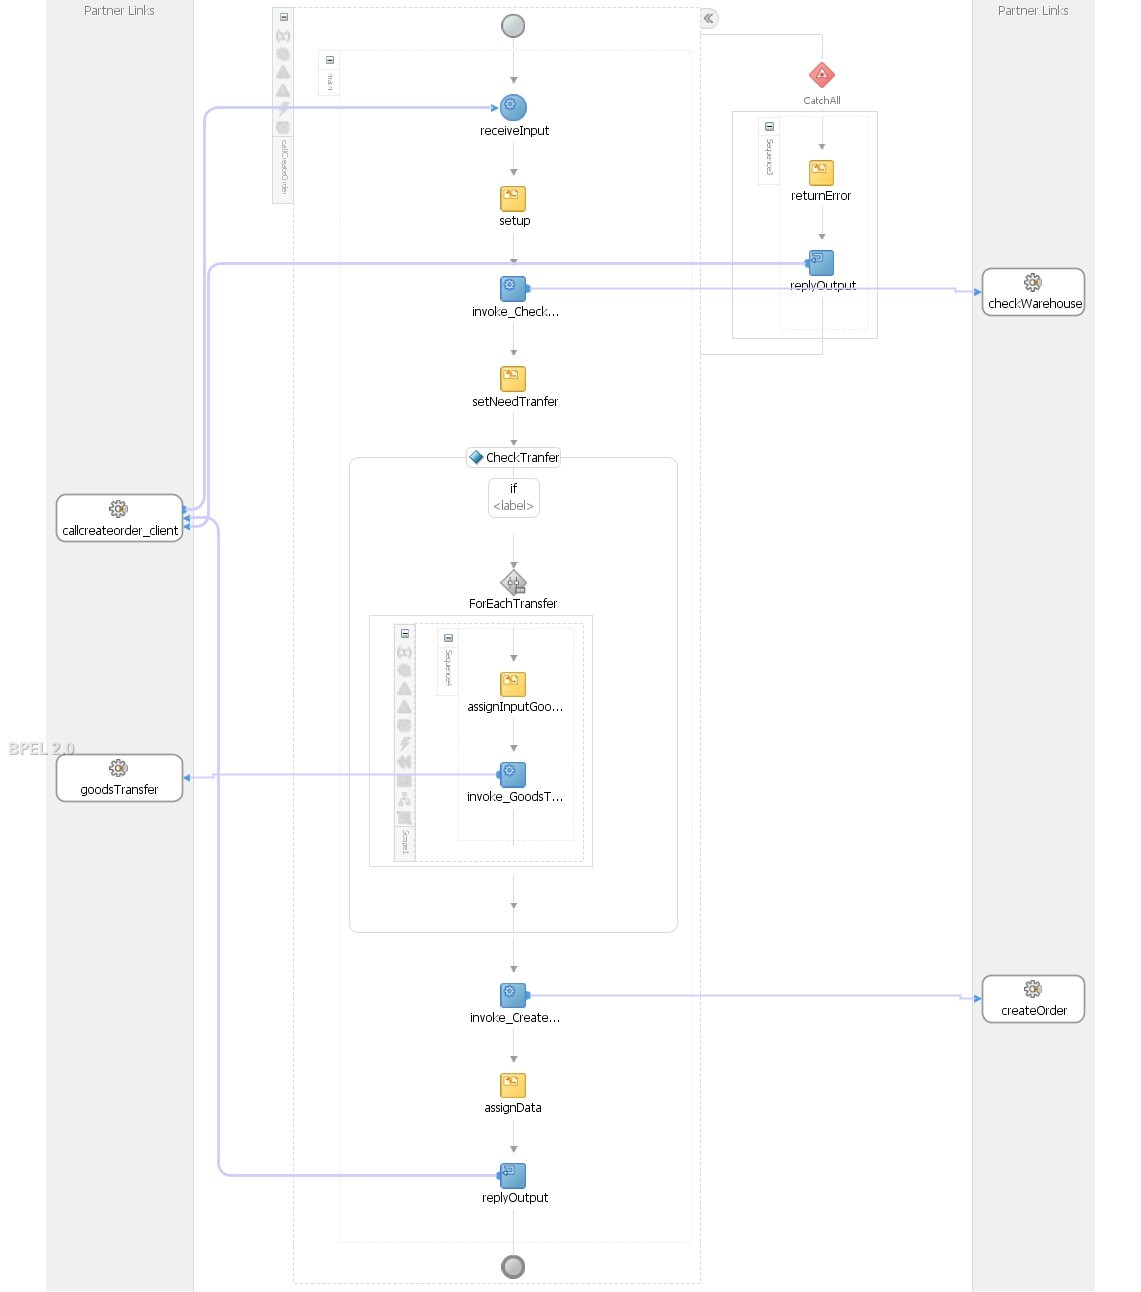
\includegraphics[width=14cm]{img/bpel/createOrderAfter.jpg}
    \newline
    \caption{Quy trình tạo đơn hàng sau khi thay đổi}
\end{figure}